%% !!!! USE PDFLaTeX to compile !!!
\documentclass[a4paper]{article}

%% \usepackage[UTF8]{ctex} % can be used for LuaLaTex
% Chinese characters:
\usepackage{CJKutf8}

\usepackage{indentfirst} % package for indent for the first line of the paragraph in the section
\usepackage{lipsum} % package for default text (= text-"template")

\usepackage{graphicx} % package for images
\usepackage{subcaption} % package for multiple images together

\usepackage{amsmath} % package for correct work of equation*
\usepackage[colorlinks=true, allcolors=blue]{hyperref} % package for colored links

%Added in file 3:
\usepackage{multirow} % package to merge rows
\usepackage{diagbox} % package for diag lines

\begin{document}
\pagenumbering{gobble} % exclude page numbering since current page
\begin{center}

{\Huge 
This is Title Page
}
\vspace{10cm} % add indent between lines

\LARGE Hangzhou

\begin{CJK*}{UTF8}{gbsn} % add Chinese characters
文章内容。

基于宏的流行的文本格式化程序
\end{CJK*}

2020
\rm % clear font of the text
\end{center}

\newpage % start new page
\pagenumbering{arabic} % set page number style
\setcounter{page}{2} % set number of the current page

\section{Part 1. Lipsum}

Hello, world!

\lipsum[7] % 7th paragraph
\medskip % small indent between lines 
\lipsum[10] % 10th paragraph
\bigskip % big indent between lines
\lipsum[7-10] % Paragraphs 7-10


\newpage
\section{Part 2. Pictures, formulas}
\subsection{Pictures}

There are multiple ways to modify the size of the picture~\ref{fig:Label_cat}.

\begin{figure}[h] % = hit there
    \centering
    
\includegraphics[scale=0.2]{Shrek.jpg}
    \caption{Shrek cat}
    \label{fig:Label_cat}
\end{figure}

\begin{figure}[b] % bottom of the document
 
    \begin{subfigure}{0.5\textwidth}
    \centering
    
\includegraphics[width=0.5\linewidth, height=9cm]{Shrek.jpg} 
    \caption{Cat}
    \label{fig:subim1}
    \end{subfigure}
    \begin{subfigure}{0.5\textwidth}
    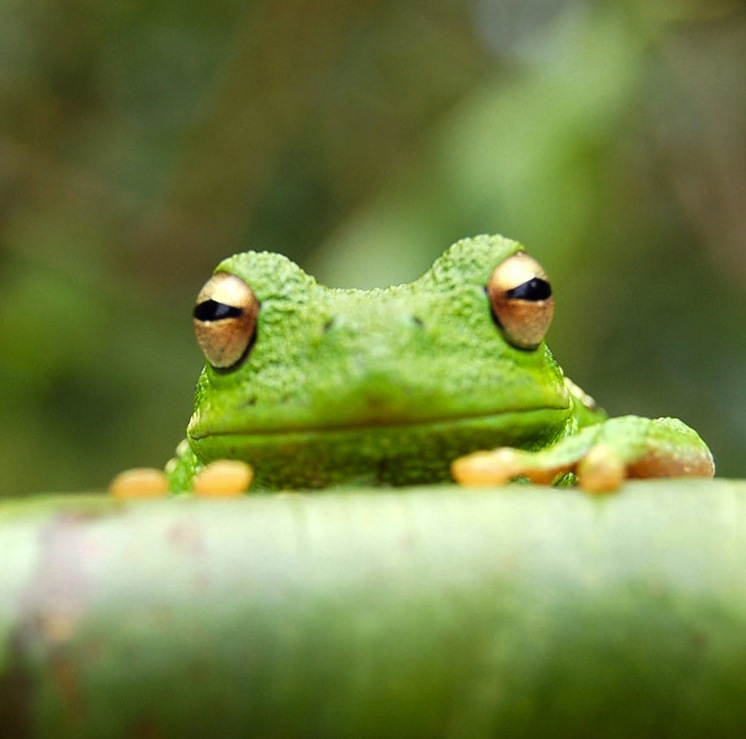
\includegraphics[width=0.9\linewidth, height=2cm]{frog.jpg}
    \caption{Frog}
    \label{fig:subim2}
    \end{subfigure}
 
\caption{Cat and frog}
\label{fig:zoo}
\end{figure}

\subsection{Formulas}

\vspace{4cm}

Identify the difference between formulas:
\bigskip

\hrule
\medskip

\large

$(a+x)^r=a^r+ra^(r-1)x+\frac{r(r-1)}{1*2}ax^2$

\bigskip

$(a+x)^r=a^r+ra^{r-1}x+\frac{r(r-1)}{1*2}ax^2$

\begin{equation}
(a+x)^r=a^r+ra^{r-1}x+\frac{r(r-1)}{1*2}ax^2    
\label{eq:Example1}    
\end{equation}

\begin{equation*}
(a+x)^r=a^r+ra^{r-1}x+\frac{r(r-1)}{1*2}ax^2    
\label{eq:Example2}    
\end{equation*}

\bigskip
The formula~\ref{eq:Example1} is very helpful.

But the formula~\ref{eq:Example2} is not.


\[S_n = \int_{-\infty}^{+\infty}\frac{X_1 + X_2 + \cdots + X_n}{n}
      = \frac{1}{n}\sum_{i}^{n^{12*21}} X_i\]

\vspace{2cm}

\textbf{PERSONAL TASK 1}
\bigskip
\rm

Create the expression for the formula presented on the picture~\ref{fig:Pers_Task_1}:

\begin{figure}
    \centering
    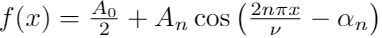
\includegraphics[scale=1.1]{Formula}
    \caption{Formula for personal task 1}
    \label{fig:Pers_Task_1}
\end{figure}

%https://tex.stackexchange.com/questions/17611/how-does-one-type-chinese-in-latex

\hrule
\vspace{1cm}

!!! YOU SHOULD SUBSTITUTE THIS TEXT WITH THE EXPRESSION ACCORDING TO PERSONAL TASK 1 !!!

\newpage
\section{Part 3. Lists, tables}
\subsection{Lists}

In general there are 2 lists' types in \TeX: unordered (unnumbered) and ordered.

 \begin{itemize}
   \item  First Level
   \begin{itemize}
     \item  Second Level
     \begin{itemize}
       \item  Third Level
       \begin{itemize}
         \item  Fourth Level
       \end{itemize}
     \end{itemize}
   \end{itemize}
 \end{itemize}
 
 \bigskip
 
 \begin{enumerate}
   \item First level item
   \item First level item
   \begin{enumerate}
     \item Second level item
     \item Second level item
     \begin{enumerate}
       \item Third level item
       \item Third level item
       \begin{enumerate}
         \item Fourth level item
         \item Fourth level item
       \end{enumerate}
     \end{enumerate}
   \end{enumerate}
 \end{enumerate}

You can use combination of them. Create by yourself.

\vspace{3cm}
\subsection{Tables}

There are many ways to create a table. Examples below have combined columns, rows, diag lines:

\begin{center}
\begin{tabular}{|c|c|c|c|c|c|c|}
\cline{3-7}
\multicolumn{2}{c|}{} & \multicolumn{4}{c|}{Values} & \multirow{2}{*}{Total} \\ \cline{3-6}
\multicolumn{2}{c|}{} & A & B & C & D & \\ \hline
\multirow{2}{*}{Range} & min & 4 & 8 & 15 & 16 & 43 \\ \cline{2-7}
                       & max & 23 & 42 & 25 & 34 & 124 \\ \hline
\multicolumn{2}{|c|}{Another total} & 27 & 50 & 40 & 50 & \textbf{167} \\ \hline
\end{tabular}\\


\vspace{1em}


\begin{tabular}{c|>{\bfseries}c|c|>{\itshape}c|c|c}
\diagbox{n}{k} & 0  & 1 & 2 & 3 & 4 \\ \hline 
0 & 1 & 0 & 0  & 0  & 0 \\ \hline
1 & 1 & 1 & 0  & 0  & 0 \\ \hline
2 & 1 & 2 & 1  & 0  & 0 \\ \hline
3 & 1 & 3 & 3  & 1  & 0 \\ \hline
4 & 1 & 4 & 6  & 4  & 1 \\ \hline
5 & 1 & 5 & 10 & 10 & 5 \\  
\end{tabular}
\end{center}


\vspace{2cm}

\textbf{PERSONAL TASK 2}
\bigskip
\rm

Create a table to be the same as the table presented on the picture~\ref{tab:Pers_Task_2}:

\begin{figure}
    \centering
    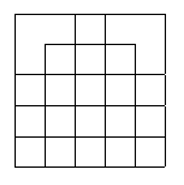
\includegraphics[scale=1]{Table}
    \caption{Table for personal task 2}
    \label{tab:Pers_Task_2}
\end{figure}


\end{document}